\section{Experiment}

% -------- section structure ----------
%    (a) description of jlab facility, cebaf, overview of the entire process 
%    (b) description of beam, helicity and energy 
%    (c) description of target used 
%    (d) description of detector systems 
%    (e) electron identification 
%    (f) hadron identification 
% ------------------------------------

% general description of jlab, cebaf, and the experiment
This measurement was conducted at Jefferson Lab in Newport News, Virginia.  Jefferson Lab houses the Continuous Electron Beam Accelerator Facility (CEBAF), as well as 4 experimental halls.  The data used for this study was taken with the CEBAF Large Acceptance Spectrometer (CLAS) in Hall-B during 6 GeV operation.  \\

\begin{figure}
  \label{fig:clas}
  \begin{center}
    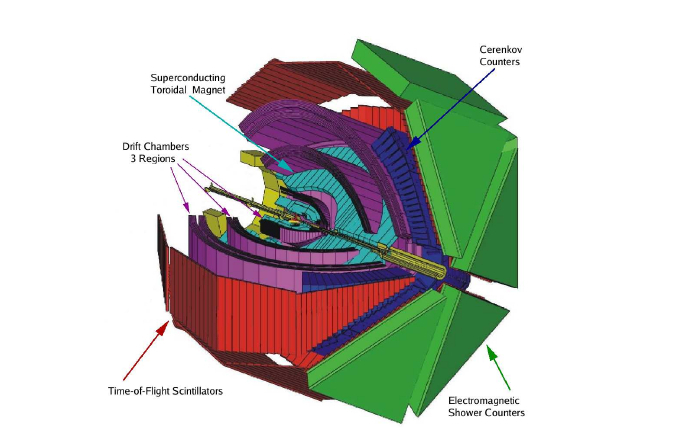
\includegraphics[width=\columnwidth]{image/clas.png}
    \caption{CLAS Detector shown with sub-systems labeled.}
  \end{center}
\end{figure}

% description of the beam properties (helicity and energy)
%The CEBAF injector provides a few hundered (get the number and put it here) MeV electrons, where a high voltage Pockels cell is used to switch the polarization of the electrons at a rate of 33 Hz.  Electrons are then accelerated via several passes through 2 parallel linear accelerators, before being delivered to Hall-B.  

% discussion of the detector systems and clas 
The CLAS detector is composed of several sub-systems that are used together to infer the four momenta of particles that scatter out of the target.  A central magnet provides a toroidal magnetic field used to separate charged particles and measure momentum, and divides the spectrometer azimuthally (in the x-y plane if z is taken to be the direction of the beam) into 6 identically constructed sectors.  Each sector contains 4 major sub-systems: 

\begin{itemize}
	\item Drift Chambers - Used to detect tracks from charged particles and measure the particle momentum.  Also responsible for most of the trajectory tracking of the particles.
	\item Cherenkov Counter - Used to separate electrons from negative hadrons.
	\item Electromagnetic Calorimeter - Records the energy deposited by charged and neutral particles, resposible for tracking photons/neutrons.
	\item Time of Flight Scintillators - A high resolution timing system that is used to calculate the velocity of particles.  The time of flight system is the primary means used to separate different hadrons.  
\end{itemize}

For the E1-F experimental run the beam energy was 5.5 GeV.  The beam polarization was monitored with a Moller polarimeter, and the average value was found to be $\lambda_e = (75 \pm 3) \%$.  The electron beam was incident on a liquid hydrogen target, 5 centimeters in length. \\

% electron identification 
\subsection{Electron Identification}
Electrons are selected for analysis from the candidate tracks by using a cuts based classification algorithm.  The dominant background for electron candidates are negative pions.  All negative tracks are considered as possible electrons.  These candidate electrons are first subject to geometric cuts.  
\\

\begin{figure}
  \label{fig:sampling_fraction}
  \begin{center}
    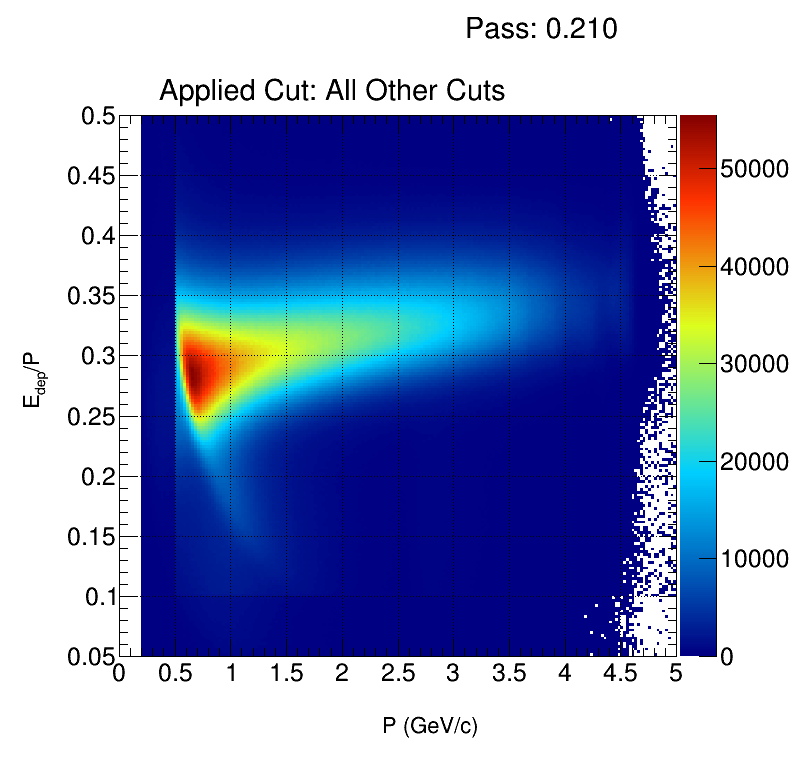
\includegraphics[width=10cm]{image/h_etot_p_allOthers_all.png}
    \caption{Sampling fraction for electron candidates (all other cuts passed).}
  \end{center}
\end{figure}

As particles traverse the EC they create an electromagnetic shower, which is not confined within the detector when the particles pass close to the extremes of the detector strips.  This mechanism leads to an underestimation of particle energy in the reconstruction phase, for that reason these tracks are discarded.  Similarly, the detector efficiency is poorly understood at the extreme edges of the drift chambers, and tracks through these areas are also rejected.  \\

The fractional energy deposition with respect to the particle momentum $E_{dep}/p$ is nearly constant as a function of momentum for electrons, but inversely depends on the momentum for negative pions.  This property is exploited by placing a momentum dependent cut on the ratio $E_{dep}(p)/p$ for all negative candidate tracks.  The ratio $E_{dep}/p$ is calculated in 60 momentum bins from 0.5 to 2.5 GeV/c (this should be double-checked).  The electron signal is then fit with a Gaussian function, and the mean $\mu_i$ and standard deviations $\sigma_i$ are recorded for each momentum bin (above labeled i).  These distributions are then fit with a 3rd order polynomial ($\mu(p) = ap^3 + bp^2 + cp + d$) and can be used to create decision boundaries for rejecting tracks from the candidate electron sample.  
\\

\begin{figure}
  \label{fig:ec_edep}
  \begin{center}
    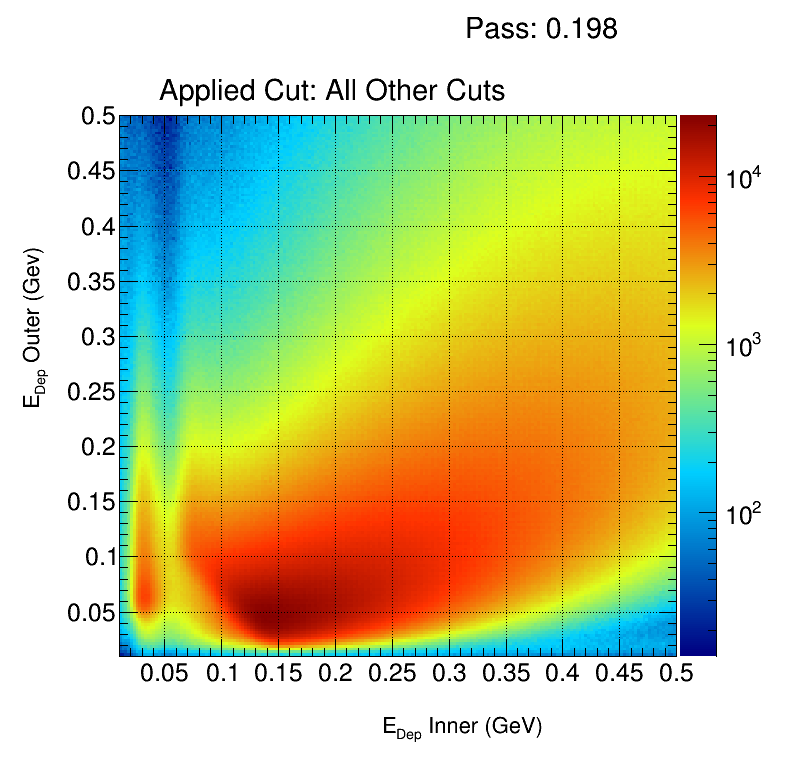
\includegraphics[width=10cm]{image/h_ec_edep_allOthers_all.png}
    \caption{Calorimeter energy deposition for electron candidates (all other cuts passed).}
  \end{center}
\end{figure}

Unlike electrons, negative pions do not deposit a significant amount of energy in the inner EC, and we apply a minimum energy deposition cut to electron candidates ($E_{inner} > 50 MeV$).  The Cherenkov Counter (CC) is filled with $C_{4}F_{10}$ gas (perfluorobutane), which has a pion threshold of $p_{\pi} \approx 2.5 GeV/c$.  Historically, a cut was placed on the minimum number of photo-electrons detected for a track.  This cut achieves the desired separation between electrions and negative pions, but is known to discard good electron candidates as well.  For this analysis, we use a matching condition developed by Osipenko.  Using the closest detector (drift chamber region 3) the track polar angle is calculated at the CC.  This angle is compared with the CC detection segment for each of the 18 segments which span the polar angle up to $\theta = 45^{\circ}$.  The procedure described above for fitting the momentum dependence of the ratio $E_{dep}/p$ is applied to the segment dependence of the angle $\theta_{CC}$.  
\\
\subsection{Positive Pion Identification}

After electron identification, all positive tracks are subject to two constraints.  First, events which pass close to the torus coils are removed by cutting on the hit positions reported by the region 1 drift chambers, this is shown in figure \ref{fig:fid}.  Such events are often poorly reconstructed or have poorly understood acceptances and are discarded from analyses.  Then, the distance between the electron vertex and the positive track vertex is computed ($\delta v_{z} = v_{z}^{e} - v_{z}^{+}$).  This distance is constrained to be within the length of the target (5 cm) see figure \ref{fig:dvz}.  

\begin{figure}
  \label{fig:dvz}
  \begin{center}
    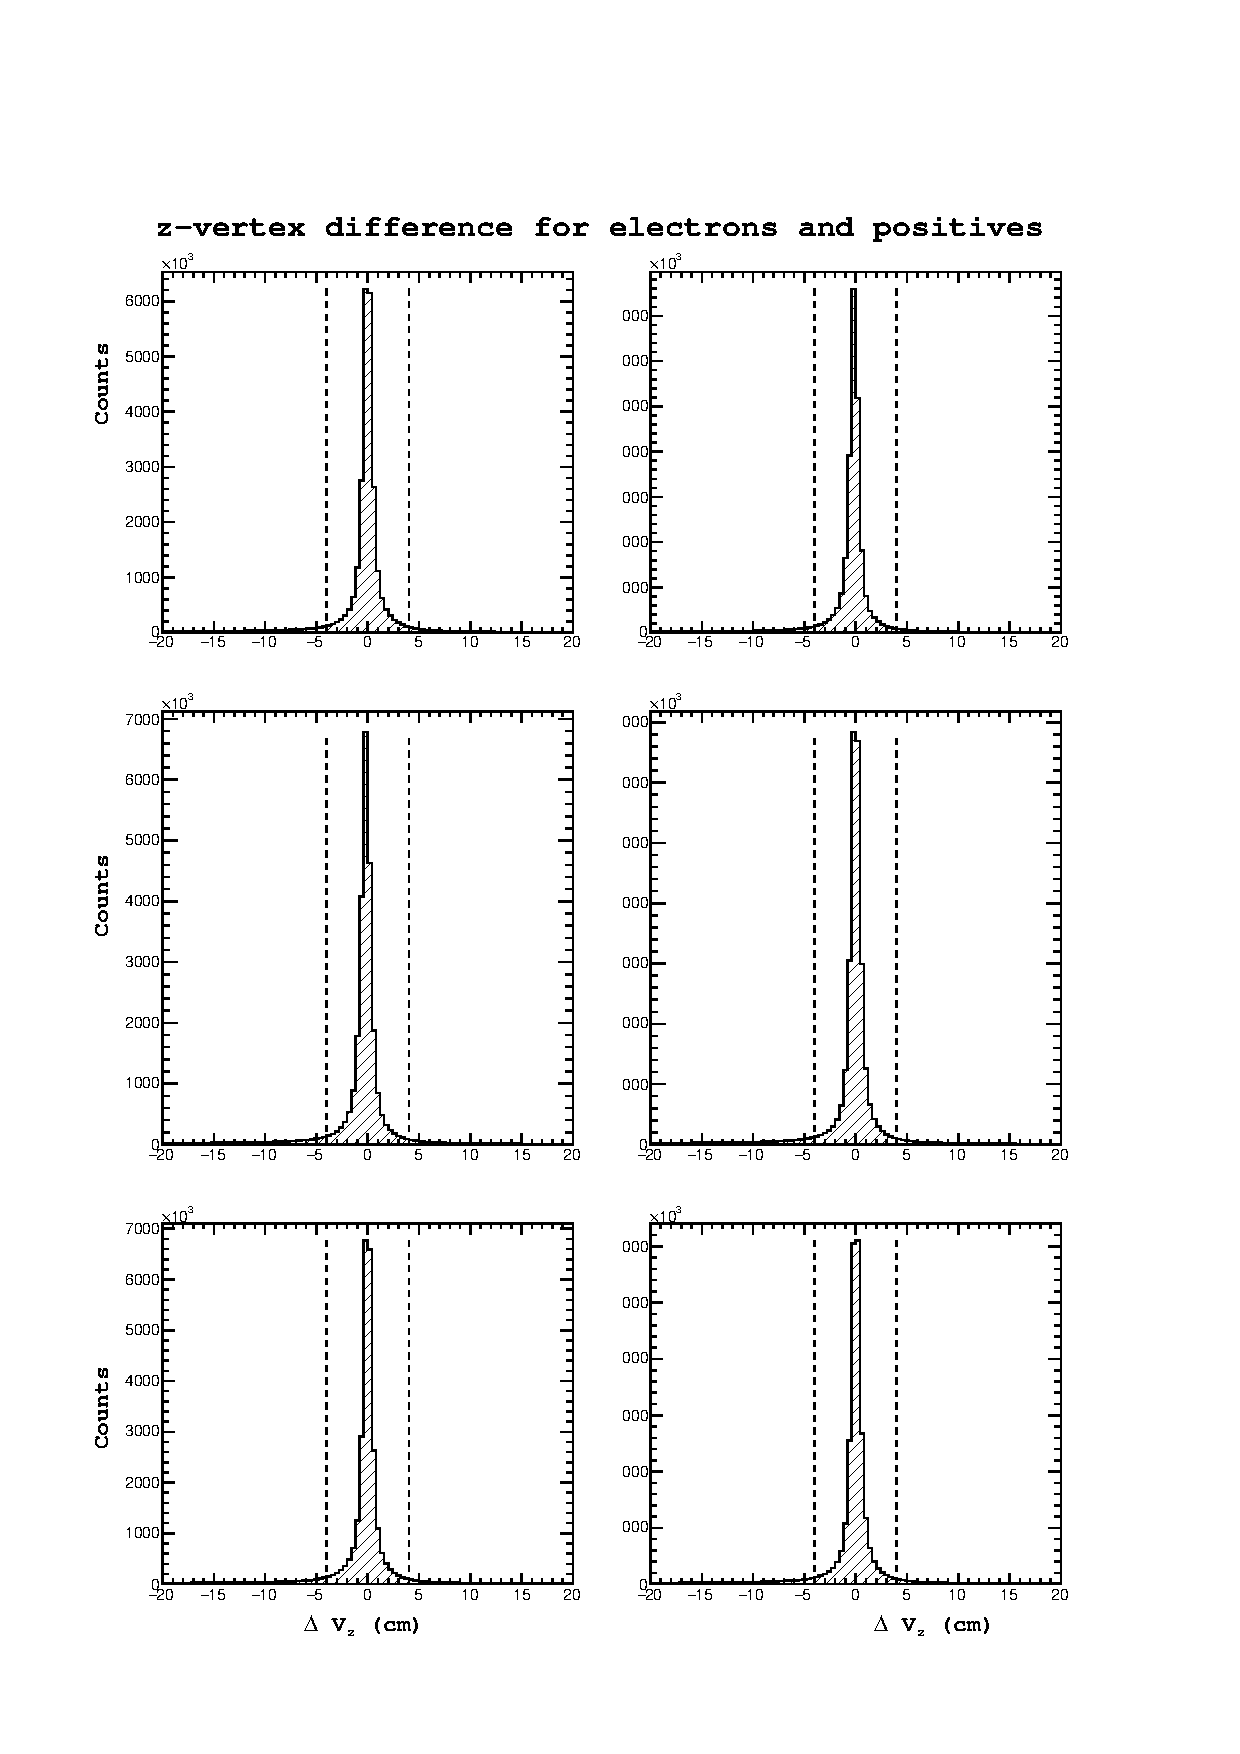
\includegraphics[width=10cm]{image/dvz.pdf}
    \caption{Shown above: The difference between the z-vertex position between detected electrons and positive tracks.}
  \end{center}
\end{figure}

\begin{figure}
 \label{fig:fid}
  \begin{center}
    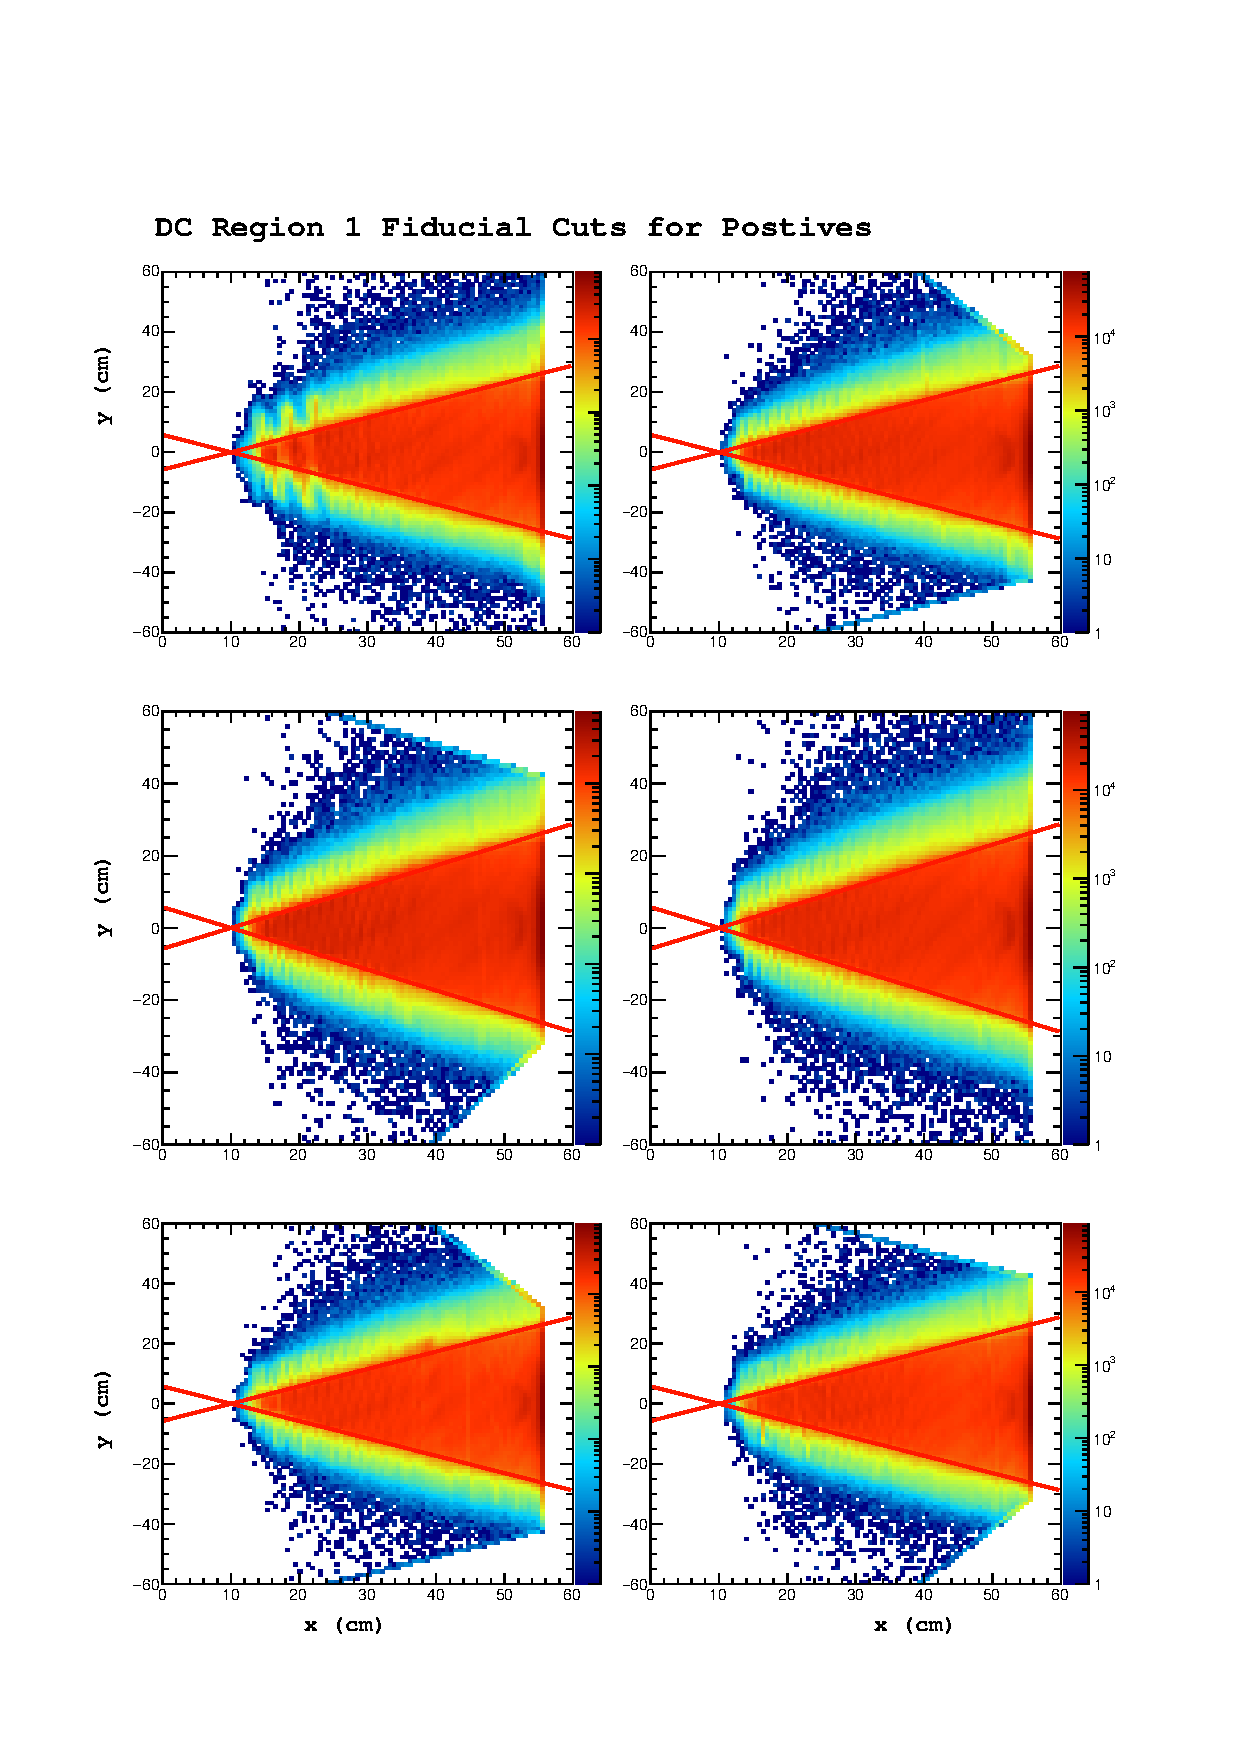
\includegraphics[width=10cm]{image/fid.pdf}
    \caption{Shown above: Positive track hits on the region 1 drift chamber, events falling between the red lines are kept for analysis.}
  \end{center}
\end{figure}

\begin{figure}
  \label{fig:pbeta}
  \begin{center}
    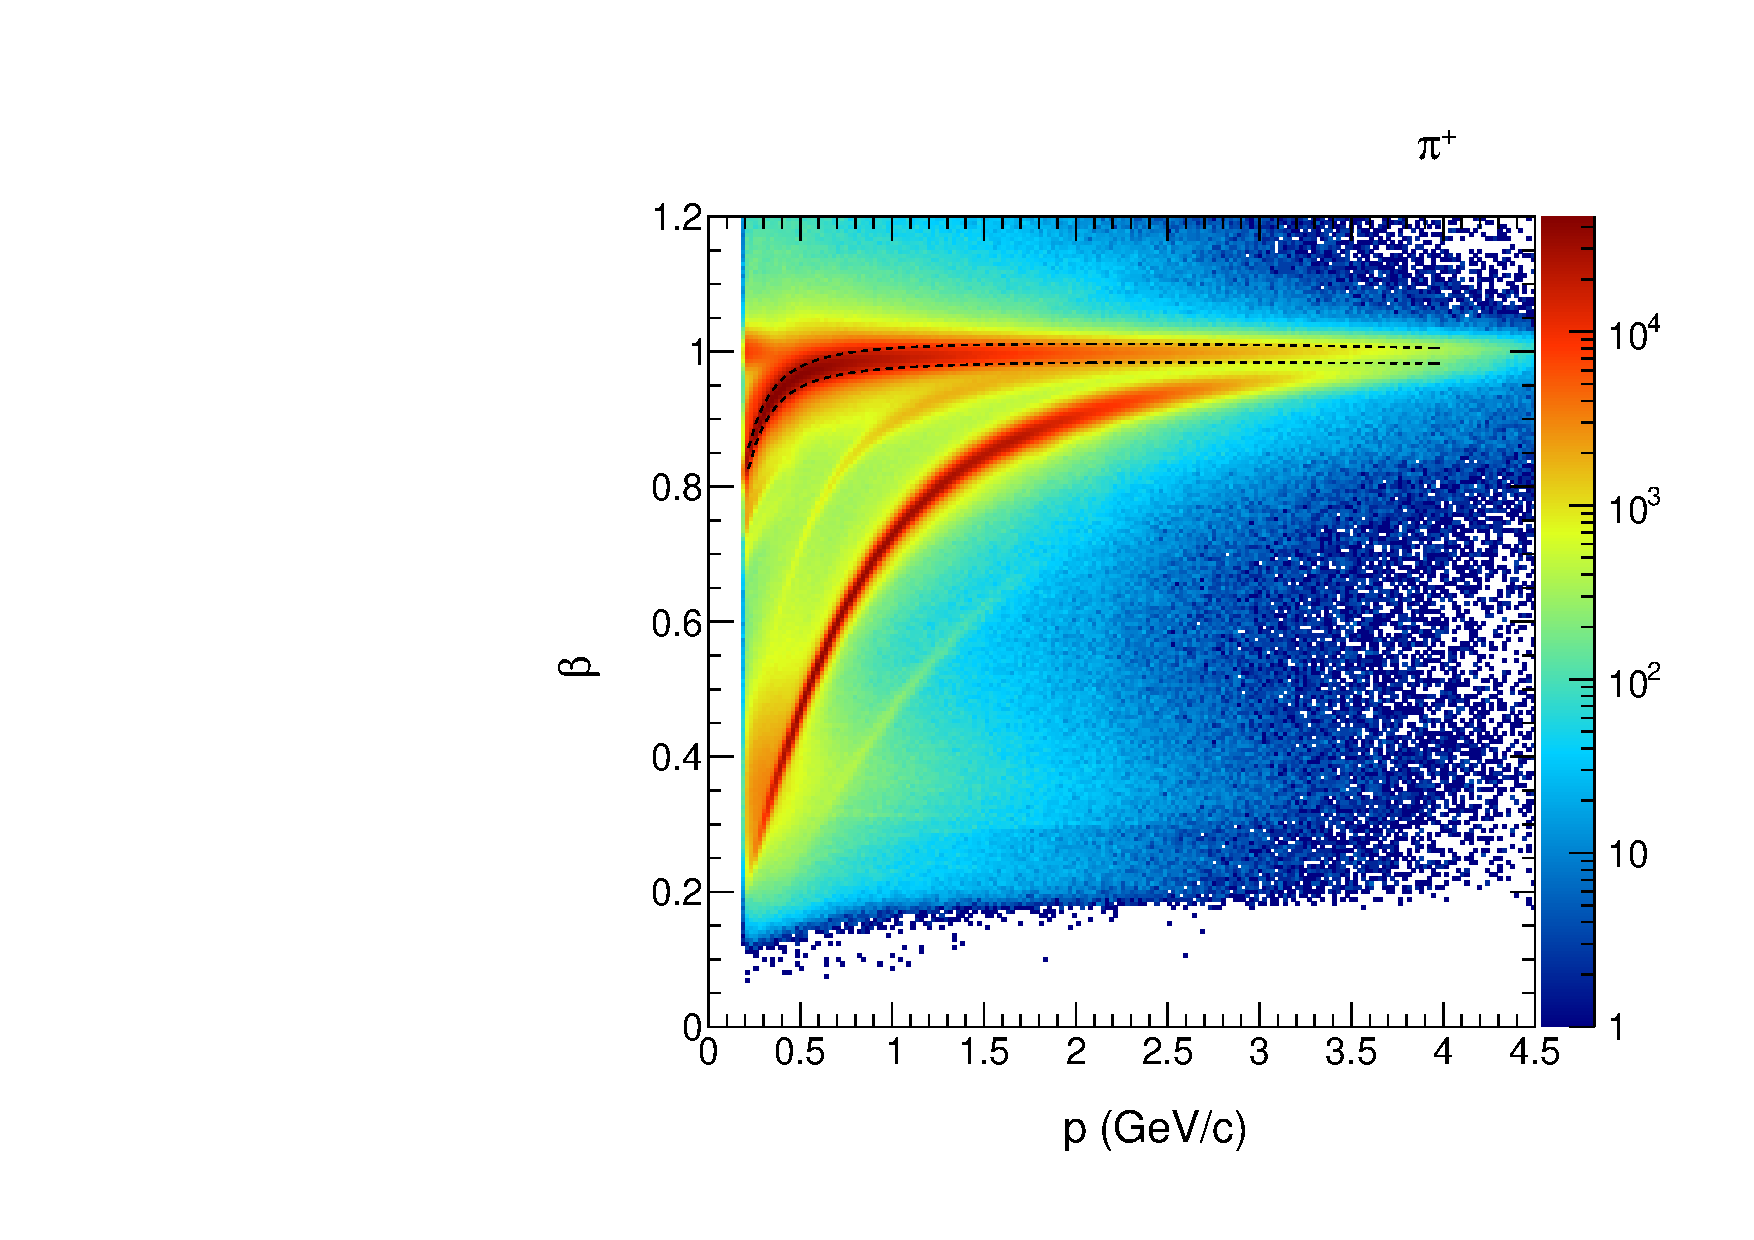
\includegraphics[width=10cm]{image/beautiful_pbeta_pip.pdf}
    \caption{$\beta(p)$ resolution for positive pions shown.}
  \end{center}
\end{figure}

\subsubsection{Likelihood Method}

For each particle species considered, a normalized probability density function $P(x;p,h)$ is constructed for each input into the likelihood analysis.  Here, x corresponds to the feature being used to catagorize different particles (in our case, x is the $\beta$ value measured by CLAS time-of-flight), p is the particle momentum, and h is the hadron being hypothesized (eg: in our case the possible values for h are pion, kaon, proton).  In general if one uses a set of $N$ variables $x = (x_1, x_2, ..., x_N)$, the likelihood for a hypothesis h is defined below.

\begin{equation}
  \mathcal{L}_h = \prod^{N}_{i=1} P_{i} (x_i; p, h)
\end{equation}

In our case, the only random variable we consider is $\beta$, and the likelihood is just the PDF.  Here, and in many cases where the choice is statistically appropriate, it is possible to use a Gaussian PDF for the variable $x_i$ ($\beta$).

\begin{equation}
  P(\beta;p,h) = \frac{1}{\sqrt{2 \pi} \sigma_\beta(p,h) } exp \left \{ -\frac{1}{2} \bigg( \frac{\beta - \mu_\beta(p,h)}{\sigma_\beta(p,h)} \bigg)^2 \right \}
\end{equation}

The identity is assigned by choosing the particle hypothesis h which maximizes the likelihood ratio.

\begin{equation}
  \frac{\mathcal{L}_h}{\mathcal{L}_{\pi}+\mathcal{L}_{K}+\mathcal{L}_{p}}
\end{equation}

Using this method, every positive track is assigned a particle identification.  However, at times the likelihood value is quite small when compared with the maximum likelihood for that species.  This is the case for positrons which are classified by this method as positive pions, because they are the closest particle for which a hypothesis has been provided.  To avoid these situations, the significance level $\alpha$ of each track is calculated and a cut is placed on the minumum significance.  This cut can be easily varied to see how it changes the analysis result.

\begin{equation}
  \alpha = 1 - \int_{\mu-\beta_{obs}}^{\mu+\beta_{obs}} P(\beta;p,h) d\beta
\end{equation}

%\begin{figure}
%  \begin{center}
%    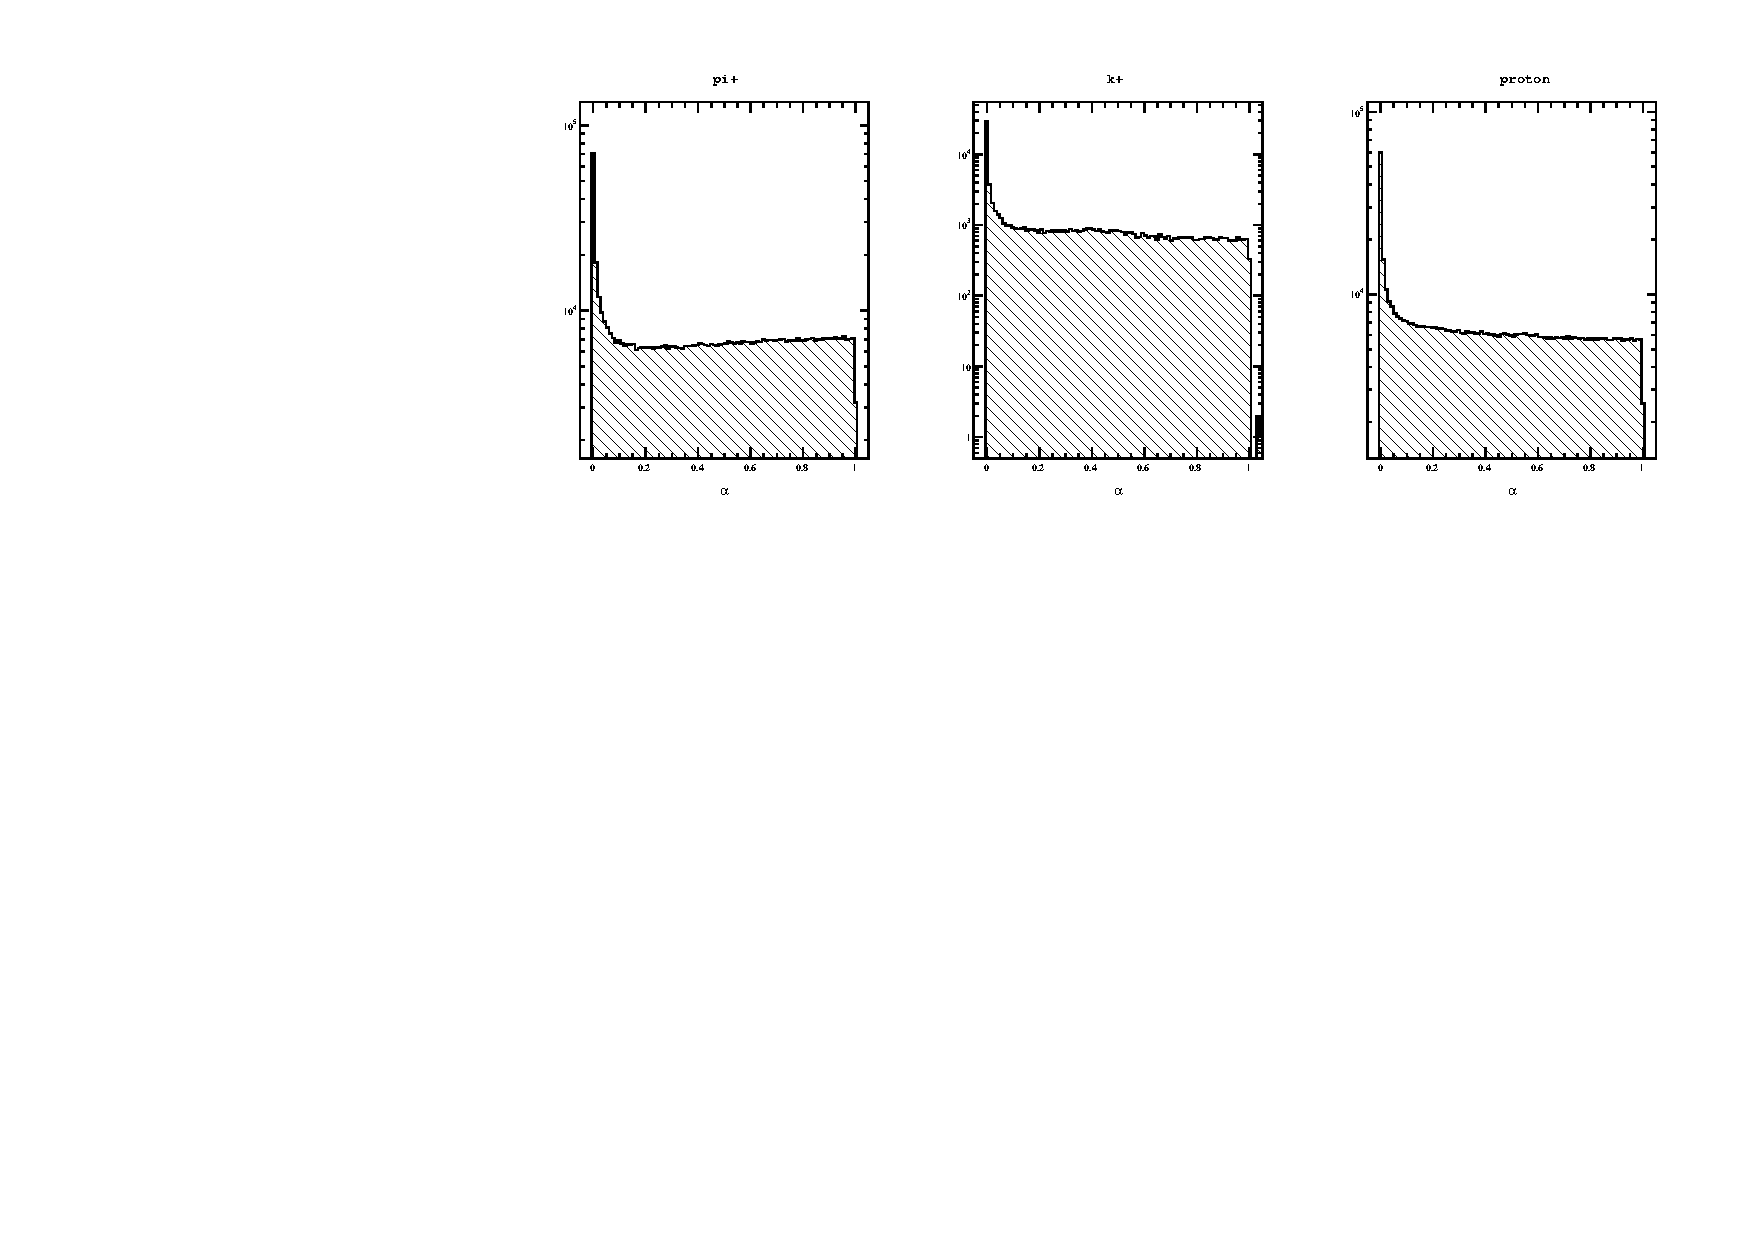
\includegraphics[width=14cm]{image/confidence_level.pdf}
%    \caption{ Shown above: The distribution of significance level for all positive tracks after being classified by the likelihood ratio.}
%  \end{center}
%\end{figure}    

Pions are chosen using this method and we apply a cut on $\alpha > 0.05$.  



